\documentclass[fleqn, a4paper, 11pt, russian]{article}

\usepackage[utf8]{inputenc}
\usepackage[T1, T2A]{fontenc}
\usepackage[english, main = russian]{babel}
\usepackage{indentfirst}
\parindent 1.27cm
\usepackage{graphicx}
\usepackage{natbib}
\usepackage{caption, subcaption}
\usepackage[top=2cm, left=2cm, right=2cm, left=2cm]{geometry}
\usepackage{amsmath} %Для работы с матрицами
\usepackage{ragged2e}
\usepackage{makecell}

\graphicspath{{Images/}}

\captionsetup[figure]{name = Рисунок, labelsep = endash}
\captionsetup[table]{name = Таблица, labelsep = endash, justification=raggedright, singlelinecheck=false}
\setlength{\mathindent}{0pt}

\begin{document}
    \newcommand\tline[2]{$\underset{\text{#1}}{\text{\underline{\hspace{#2}}}}$}

\begin{titlepage}
	\centering
	{\fontsize{12pt}{5cm}\selectfont \bfseries Министерство образования и науки Российской Федерации} \\ \vspace{0.5cm}
	{\fontsize{7pt}{5cm}\selectfont ФЕДЕРАЛЬНОЕ ГОСУДАРСТВЕННОЕ АВТОНОМНОЕ ОБРАЗОВАТЕЛЬНОЕ УЧРЕЖДЕНИЕ ВЫСШЕГО ПРОФЕССИОНАЛЬНОГО ОБРАЗОВАНИЯ} \\ 
	\vspace{1cm}
	{\fontsize{12pt}{5cm}\selectfont \bfseries САНКТ-ПЕТЕРБУРГСКИЙ УНИВЕРСИТЕТ ИНФОРМАЦИОННЫХ ТЕХНОЛОГИЙ, МЕХАНИКИ И ОПТИКИ} \\ \vspace{1.5cm}

	{\fontsize{14pt}{5cm}\selectfont Кафедра \hspace{1cm} \underline{Систем Управления и Информатики}  \hspace{1cm} Группа \underline{Р3340}} \\ 
	\vspace{2cm}

	{\fontsize{20pt}{5cm}\selectfont \bfseries Лабораторная работа №7} \\
	{\fontsize{20pt}{5cm}\selectfont \bfseries “Анализ точности систем управления”} \\
	{\fontsize{14pt}{5cm}\selectfont Вариант - 2} \\
	\vspace{1.5cm}

	\flushleft

	{Выполнил \hspace{2cm} \underline{Алякин С.П.}\tline{(фамилия, и.о.)}{6.5cm} (подпись)} \\
	\vspace{2cm}

	{Проверил \hspace{2cm} \tline{(фамилия, и.о.)}{9cm} (подпись)} \\
	\vspace{5cm}

	"\underline{\hspace{0.7cm}}"\hspace{0.2cm}\underline{\hspace{2cm}}\hspace{0.2cm}20\underline{ 17 }г. \hspace{2cm} Санкт-Петербург, \hspace{2cm} 20\underline{ 17 }г. \\ \vspace{1cm}

	Работа выполнена с оценкой \hspace{1cm} \underline{\hspace{8cm}} \\ 
	\vspace{1cm}
	Дата защиты "\underline{\hspace{0.7cm}}"\hspace{0.2cm}\underline{\hspace{2cm}}\hspace{0.2cm}20\underline{ 17 }г.
		
\end{titlepage}
    \section*{Цель работы}
    Изучение математических моделей и исследование характеристик электромеханического объекта управления, построенного на основе электродвигателя постоянного тока независимого возбуждения.
    \section*{Исходные данные}
    \begin{table}[ht!]
    	\caption{Исходные данные}
    	\begin{tabular}{| c | c | c | c | c | c | c | c | c | c |}
    		\hline
    		\makecell{$U_\text{Н},$\\В} & \makecell{$n_0,$\\об/мин} & \makecell{$I_\text{Н},$\\A} & \makecell{$M_\text{Н},$\\Н$\cdot$м} & \makecell{R,\\Ом} & \makecell{$T_\text{Я},$\\мс} & \makecell{$J_\text{Д},$\\кг$\cdot$м$^2$} & \makecell{$T_\text{У},$\\мс} & $i_\text{Р}$ & \makecell{$J_\text{М},$\\кг$\cdot$м$^2$} \\
    		\hline
    		48 & 1000 & 12 & 5,5 & 0,75 & 5 & $1,6\cdot10^{-3}$ & 6 & 16 & 2,75\\
    		\hline
    	\end{tabular}
    \end{table}
    \clearpage
    \section{Расчёт параметров математической модели двигателя}
    Переведём заданное значение частоты в систему СИ
    \begin{align}
		n_0 = 1000 \text{ об/мин} = 104,72 \text{ рад/с} = \omega_0
    \end{align}
    Рассчитаем необходимые для создания модели параметры:
    \begin{align}
    	K_\text{У} &= \frac{U_\text{Н}}{U_m} = \frac{48}{10} &= 4,8\\
    	K_\text{Д} &= \frac{1}{R} = \frac{1}{0,75} &= 1,33\\
    	K_\text{М} &= \frac{M_\text{Н}}{I_\text{Н}} = \frac{5,5}{12} &= 0,4583\\
    	K_E &= \frac{U_\text{Н}}{\omega_0} = \frac{48}{104,72} &= 0,4583\\
    	J_\text{Р} &= 0,2J_\text{Д} = 0,2 \cdot 1,6\cdot10^{-3} &= 3,2\cdot10^{-4}\\
    	J_\Sigma &= J_\text{Д} + J_\text{Р} + \frac{J_\text{М}}{i_\text{Р}^2} = 1,6\cdot10^{-3} + 3,2\cdot10^{-4} + \frac{2,75}{16^2} &= 0,01266 \text{кг}\cdot\text{м}^2
	\end{align}
	\clearpage
	\section{Вывод математической модели Вход-Состояние-Выход для полной схемы моделирования электромеханического объекта}
	Для составления математической модели запишем формулы, характеризующие ЭМО, взятые из теории к данной лабораторной работе.
	\begin{align}
		&&\begin{cases}
			T_\text{Я}\dot{I} + I = K_\text{Д}(U_\text{У} - K_E\omega)\\
			M_\text{Д} - M_C = J_\Sigma\dot{\omega}\\
			T_\text{У}\dot{U_\text{У}} + U_\text{У} = K_\text{У}U\\
			\dot{\alpha} = \omega
		\end{cases}
		\Rightarrow
		\begin{cases}
			\dot{I} = -\displaystyle{\frac{K_E}{T_\text{Я}}}\omega - \frac{1}{T_\text{Я}}I + \frac{K_\text{Д}}{T_\text{Я}}U_\text{У}\\
			\dot{\omega} = \displaystyle{\frac{K_M}{J_\Sigma}}I - \frac{1}{J_\Sigma}M_C\\
			\dot{U_\text{У}} = -\displaystyle{\frac{1}{T_\text{У}}U_\text{У}} + \frac{K_\text{У}}{T_\text{У}}U\\
			\dot{\alpha} = \omega
		\end{cases}
		,
		\label{ESETh}
	\end{align}
	где $M_\text{Д} = K_MI$.
	
	Примем вектор состояния
	$
		X =
		\begin{bmatrix}
			\alpha & \omega & I & U_\text{У}
		\end{bmatrix}^T
	$
	и вектор входных воздействий
	$
		U =
		\begin{bmatrix}
			U & M_C
		\end{bmatrix}^T,
	$
	тогда исходя из (\ref{ESETh}) получим модель Вход-Состояние-Выход:
	\begin{align}
		\begin{cases}
			\dot{X} = AX + BU\\
			y = CX
		\end{cases} \Rightarrow
		\begin{cases}
			\begin{bmatrix}
				\dot{\alpha}\\
				\dot{\omega}\\
				\dot{I}\\
				\dot{U_\text{У}}
			\end{bmatrix} =
			\begin{bmatrix}
				0 & 1 & 0 & 0\\
				0 & 0 & \displaystyle{\frac{K_M}{J_\Sigma}} & 0\\
				0 & -\displaystyle{\frac{K_E}{T_\text{Я}}} & -\displaystyle{\frac{1}{T_\text{Я}}} & \displaystyle{\frac{K_\text{Д}}{T_\text{Я}}}\\
				0 & 0 & 0 & -\displaystyle{\frac{1}{T_\text{У}}}
			\end{bmatrix}
			\begin{bmatrix}
				\alpha\\
				\omega\\
				I\\
				U_\text{У}
			\end{bmatrix}
			+
			\begin{bmatrix}
				0 & 0\\
				0 & -\displaystyle{\frac{1}{J_\Sigma}}\\
				0 & 0\\
				\displaystyle{\frac{K_\text{У}}{T_\text{У}}} & 0
			\end{bmatrix}
			\begin{bmatrix}
				U\\
				M_C
			\end{bmatrix}\\
			\alpha = 
			\begin{bmatrix}
				1 & 0 & 0 & 0
			\end{bmatrix}
			\begin{bmatrix}
				\alpha\\
				\omega\\
				I\\
				U_\text{У}
			\end{bmatrix}.
		\end{cases}
		\label{ESEFull}
	\end{align}
	
	Подставив рассчитанные ранее значения, получим следующие матрицы
	\begin{align}
		&&A = 
		\begin{bmatrix}
			0 & 1 & 0 & 0\\
			0 & 0 & 36.2 & 0\\
			0 & -91,66 & -200 & 266\\
			0 & 0 & 0 & -166,67
		\end{bmatrix}, B =
		\begin{bmatrix}
			0 & 0\\
			0 & -79,99\\
			0 & 0\\
			800 & 0
		\end{bmatrix}
	\end{align}
	\clearpage
	\section{Математическое моделирование электромеханического объекта}
	Составим математическую модель ЭМО на основе структурной схемы, представленной на рисунке \ref{fullScheme}.
	\begin{figure}[ht!]
		\centering
		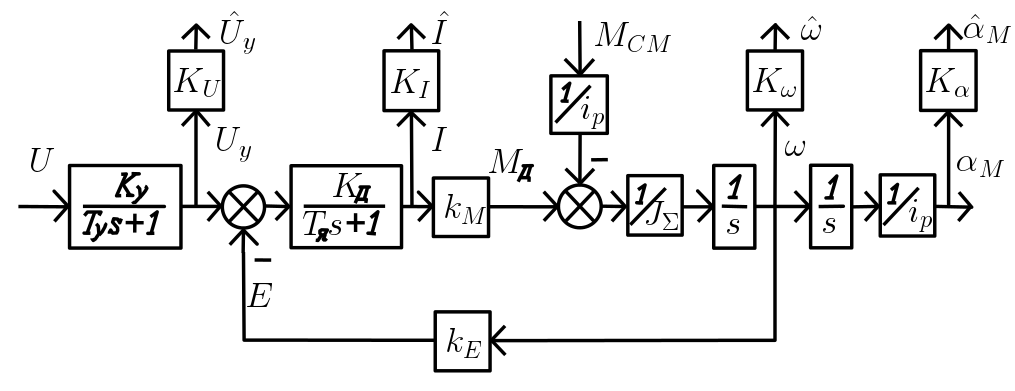
\includegraphics[width = \textwidth]{fullScheme}
		\caption{Структурная схема ЭМО}
		\label{fullScheme}
	\end{figure}
	
	Коэффициенты передачи измерительных устройств $K_U, K_I, K_\omega, K_\alpha$ выбираются таким образом, чтобы обеспечить соответствие максимального значения измеряемого сигнала уровню 10 В на выходе измерительного устройства. Из этого условия имеем:
	\begin{align}
		K_U &= 0,4175\\
		K_I &= 0,419\\
		K_\omega &= 0.19125\\
		K_\alpha &= 12
	\end{align}
	
	Схема модели представлена на рисунке \ref{fullModel}.
	\begin{figure}[ht!]
		\centering
		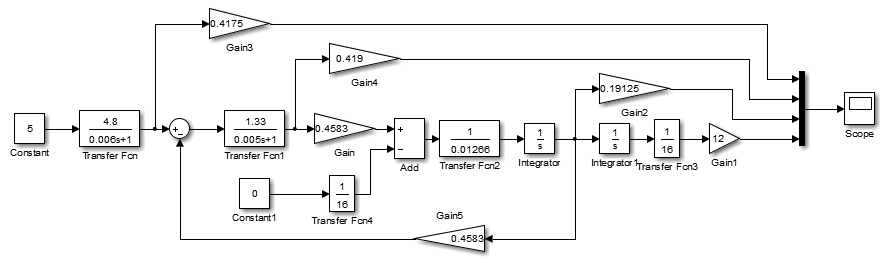
\includegraphics[width = \textwidth]{fullModel}
		\caption{Схема моделирования ЭМО}
		\label{fullModel}
	\end{figure}
	\newpage
	Построим график переходного процесса:
	\begin{figure}[ht!]
		\centering
		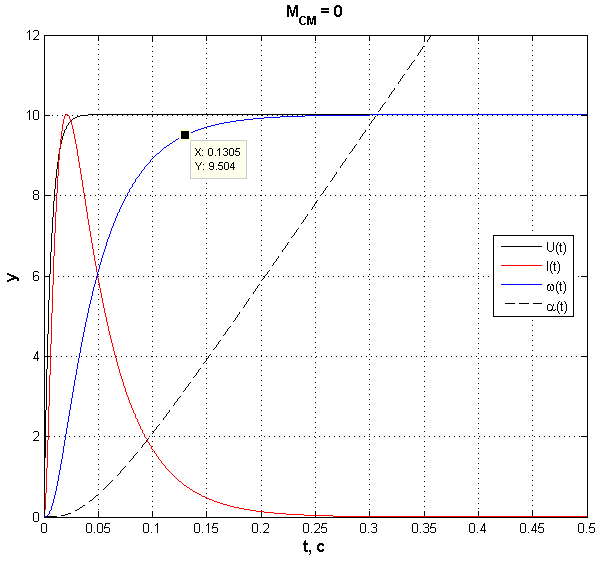
\includegraphics[width = 0.9\textwidth]{M0}
		\caption{График переходного процесса при нулевом моменте сопротивления}
		\label{M0}
	\end{figure}
	\clearpage
	\section{Исследование влияние момента сопротивления на вид переходных процессов}
	\begin{figure}[ht!]
		\centering
		\begin{subfigure}[b]{0.49\textwidth}
			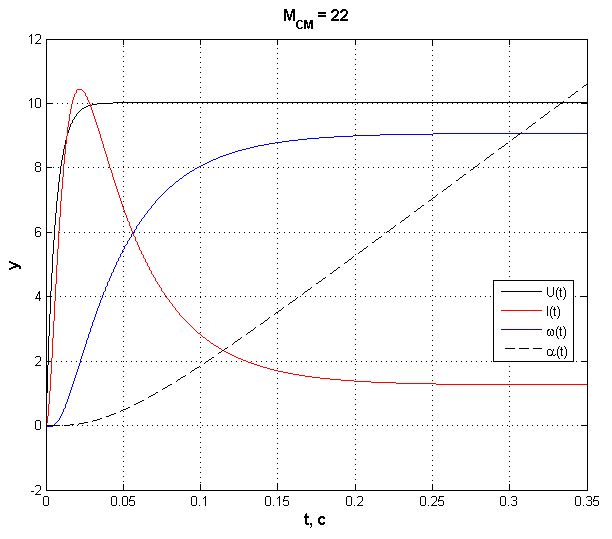
\includegraphics[width = \textwidth]{M22}
		\end{subfigure}
		\hfill
		\begin{subfigure}[b]{0.49\textwidth}
			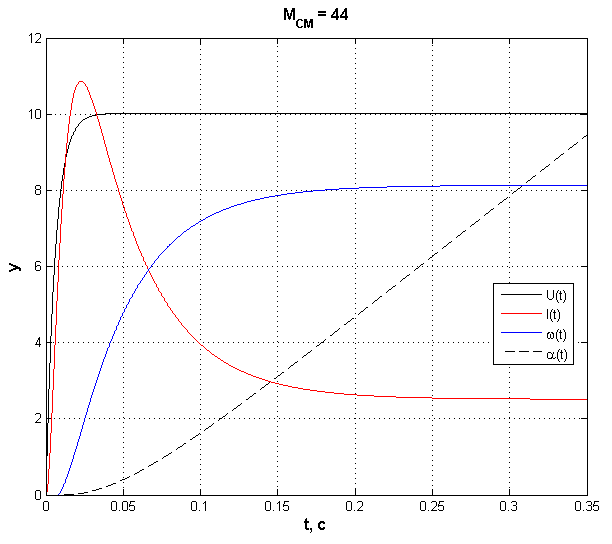
\includegraphics[width = \textwidth]{M44}
		\end{subfigure}
	\end{figure}
	\begin{figure}[ht!]\ContinuedFloat
		\centering
		\begin{subfigure}[b]{0.49\textwidth}
			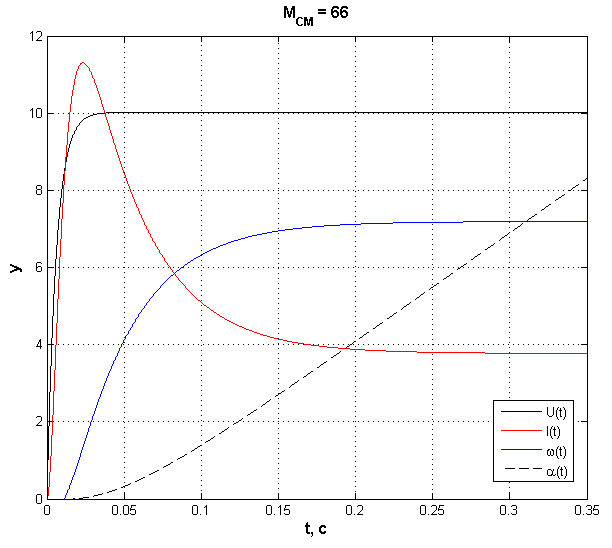
\includegraphics[width = \textwidth]{M66}
		\end{subfigure}
		\hfill
		\begin{subfigure}[b]{0.49\textwidth}
			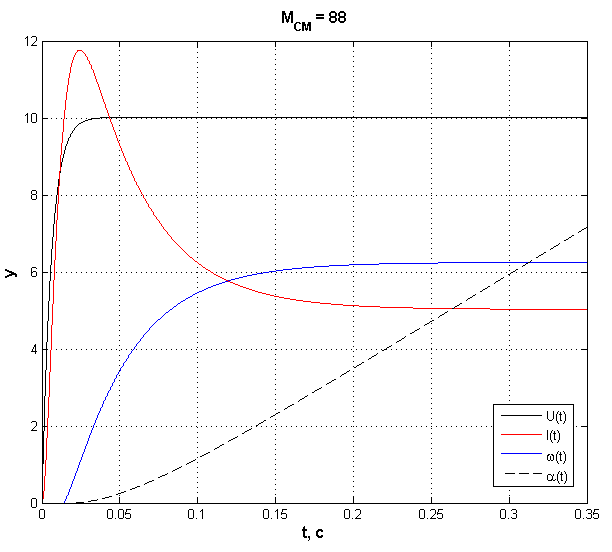
\includegraphics[width = \textwidth]{M88}
		\end{subfigure}
		\caption{Графики переходных процессов при различных значениях момента сопротивления}
		\label{MVar}
	\end{figure}
	Как видно на рисунке \ref{MVar} при увеличении момента сопротивления, время переходного процесса остаётся неизменным и равным 0,13 сек, установившееся значение скорости уменьшается, а тока --- увеличивается.
	\clearpage
	\section{Исследование влияния момента инерции нагрузки на вид переходных процессов}
	\begin{figure}[ht!]
		\centering
		\begin{subfigure}[b]{0.48\textwidth}
			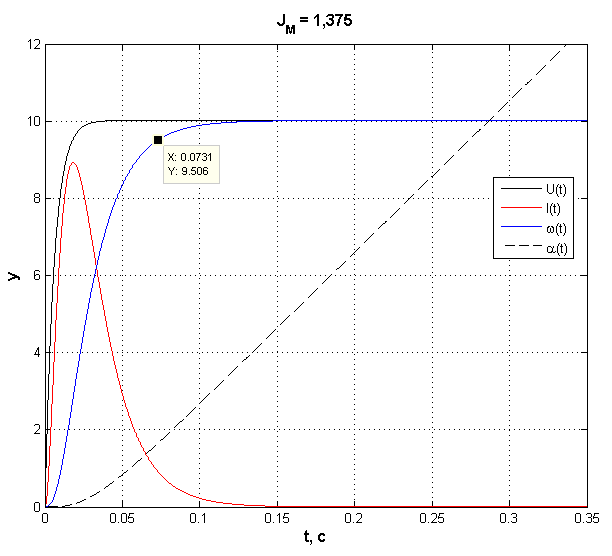
\includegraphics[width = \textwidth]{J1}
		\end{subfigure}
		\hfill
		\begin{subfigure}[b]{0.48\textwidth}
			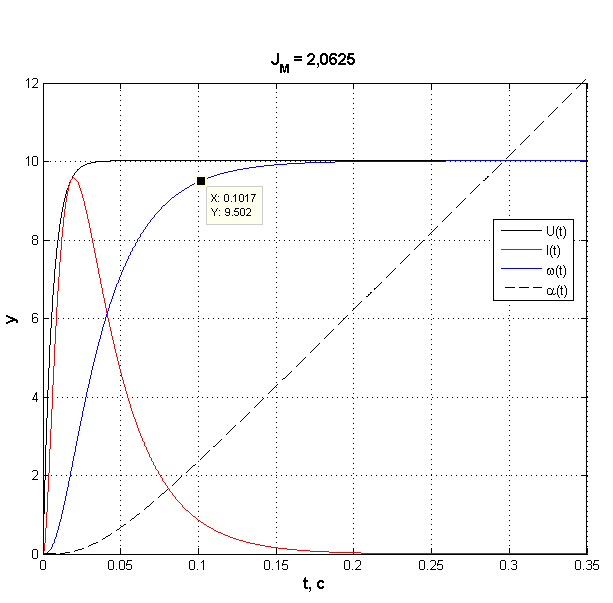
\includegraphics[width = \textwidth]{J2}
		\end{subfigure}
	\end{figure}
	
	\begin{figure}[ht!]\ContinuedFloat
		\centering
		\begin{subfigure}[b]{0.48\textwidth}
			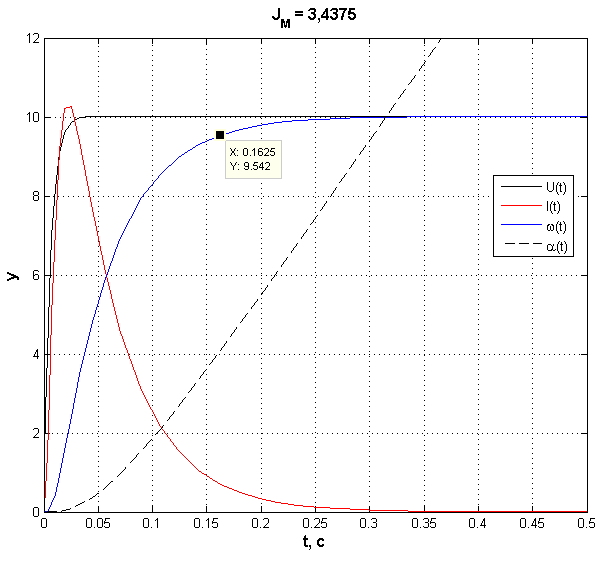
\includegraphics[width = \textwidth]{J3}
		\end{subfigure}
		\hfill
		\begin{subfigure}[b]{0.48\textwidth}
			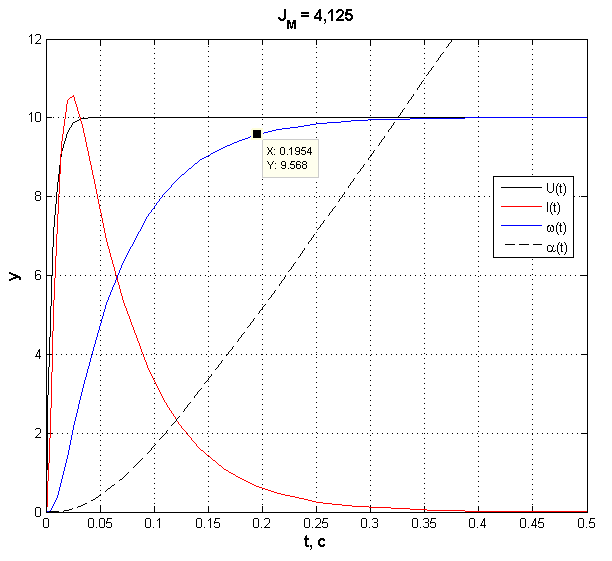
\includegraphics[width = \textwidth]{J4}
		\end{subfigure}
		\caption{Графики переходных процессов при различных значениях момента инерции нагрузки}
		\label{JVar}
	\end{figure}
	Как мы можем наблюдать на графиках переходных процессов, представленных на рисунке \ref{JVar}, время переходного процесса изменяется пропорционально с моментом инерции нагрузки $J_M$, в то время как установившиеся значения тока якоря и угловой скорости остаются неизменными.
	\clearpage
	\section{Исследование влияния передаточного момента редуктора на вид переходных процессов}
	Проведём исследования при величине момента сопротивления $M_{CM} = 0$. Их результаты приведены на рисунке \ref{M0ivar}.
	\begin{figure}[ht!]
		\centering
		\begin{subfigure}[b]{0.49\textwidth}
			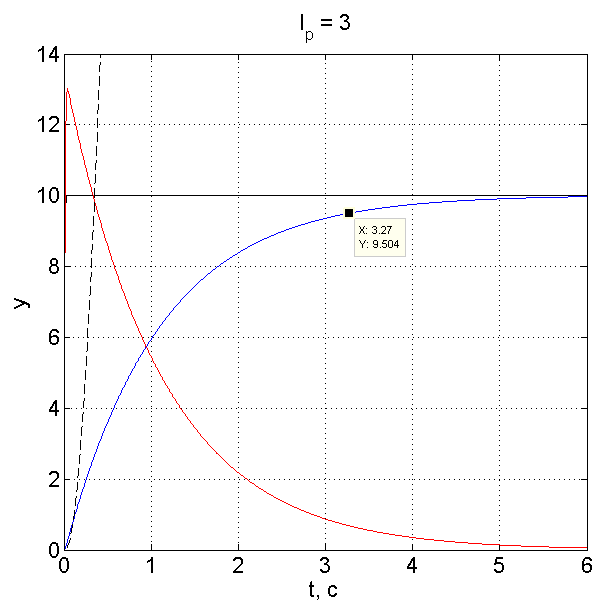
\includegraphics[width = \textwidth]{M0i3}
		\end{subfigure}
		\hfill
		\begin{subfigure}[b]{0.49\textwidth}
			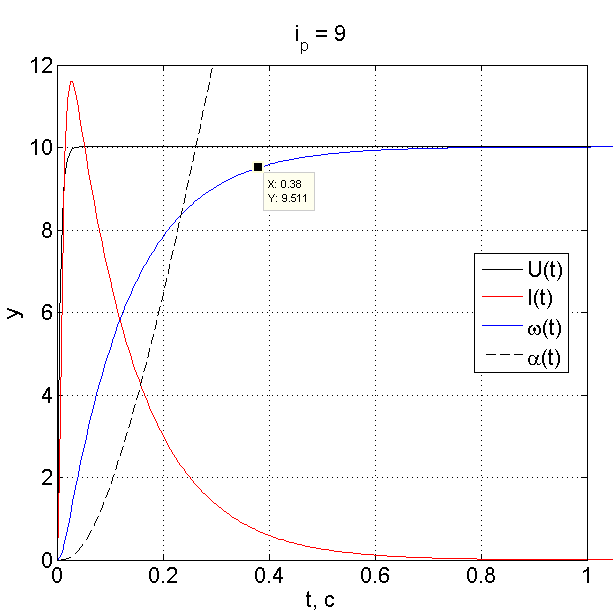
\includegraphics[width = \textwidth]{M0i9}
		\end{subfigure}
	\end{figure}
	\begin{figure}[ht!]\ContinuedFloat
		\centering
		\begin{subfigure}[b]{0.49\textwidth}
			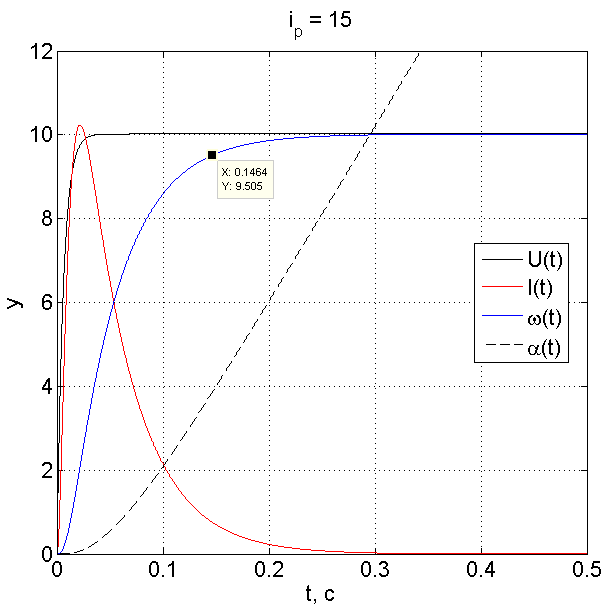
\includegraphics[width = \textwidth]{M0i15}
		\end{subfigure}
		\hfill
		\begin{subfigure}[b]{0.49\textwidth}
			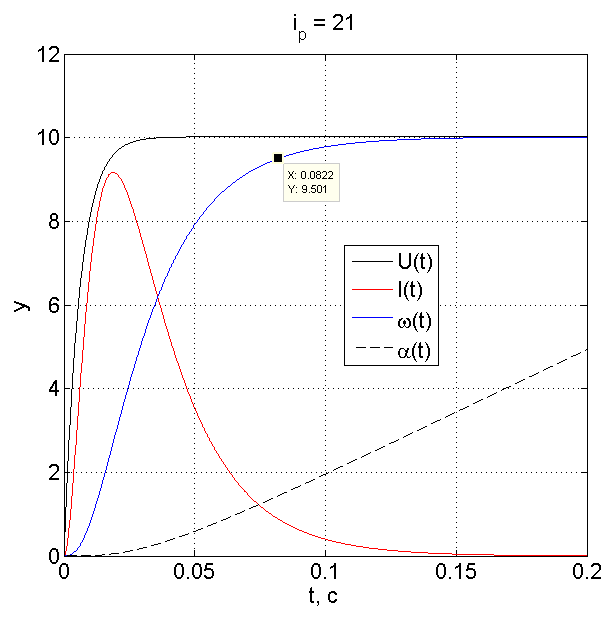
\includegraphics[width = \textwidth]{M0i21}
		\end{subfigure}
		\caption{Графики переходных процессов при нулевом моменте сопротивления и при различных значениях передаточного момента редуктора}
		\label{M0ivar}
	\end{figure}
	
	Как можно заметить по результатам математического моделирования при увеличении передаточного момента редуктора уменьшаются время переходного процесса и максимальное значение тока. Установившиеся значения тока и угловой скорости при этом остаются неизменными.
	
	Так же проведём исследования при величине момента сопротивления $M_{CM} = 44,$ что является равным половине максимального значения, рассчитанного для передаточного момента редуктора $i_p = 16$. Результаты моделирования приведены на рисунке \ref{M44ivar}.
	\begin{figure}[ht!]
		\centering
		\begin{subfigure}[b]{0.45\textwidth}
			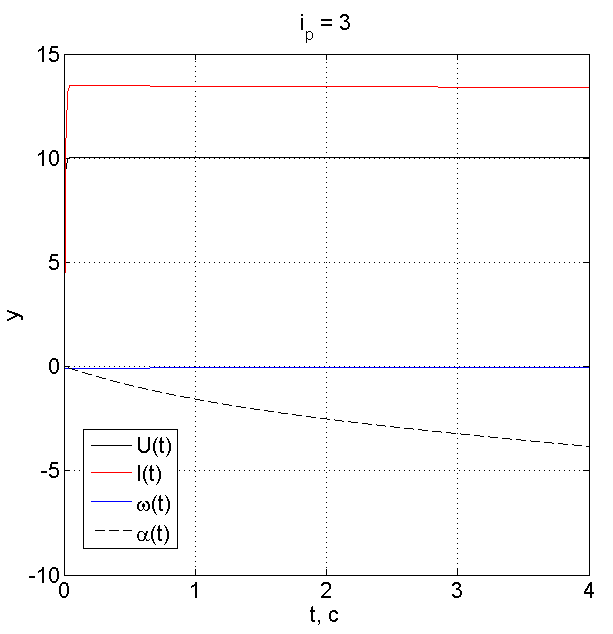
\includegraphics[width = \textwidth]{M44i3}
		\end{subfigure}
		\hfill
		\begin{subfigure}[b]{0.45\textwidth}
			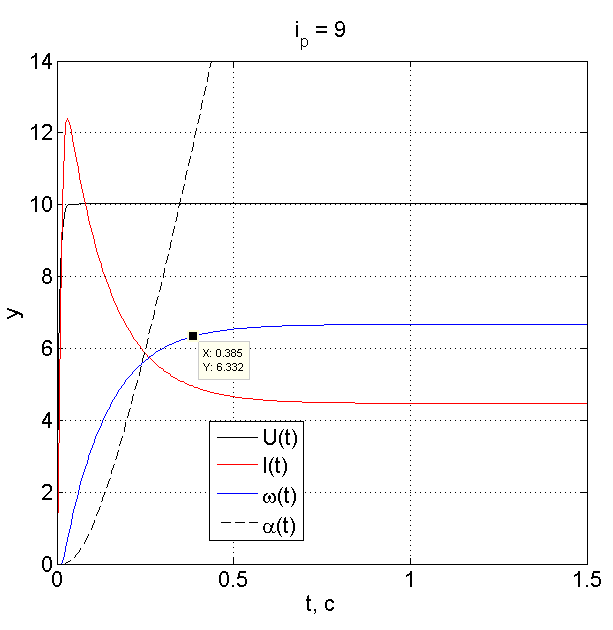
\includegraphics[width = \textwidth]{M44i9}
		\end{subfigure}
	\end{figure}
	\begin{figure}[ht!]\ContinuedFloat
		\centering
		\begin{subfigure}[b]{0.45\textwidth}
			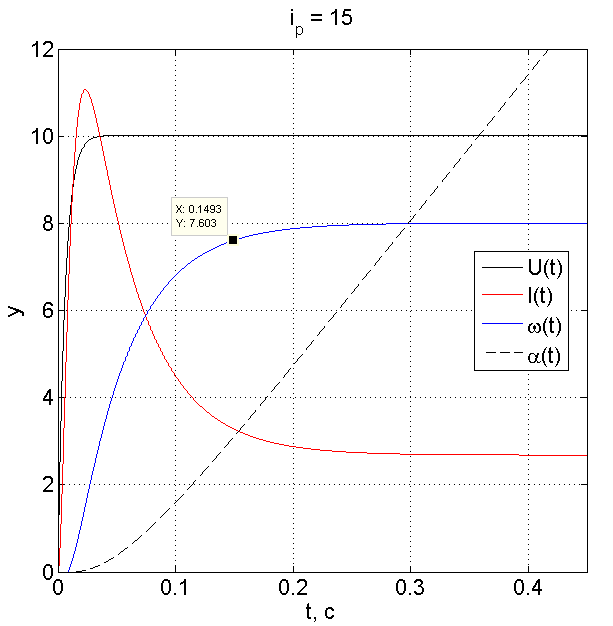
\includegraphics[width = \textwidth]{M44i15}
		\end{subfigure}
		\hfill
		\begin{subfigure}[b]{0.45\textwidth}
			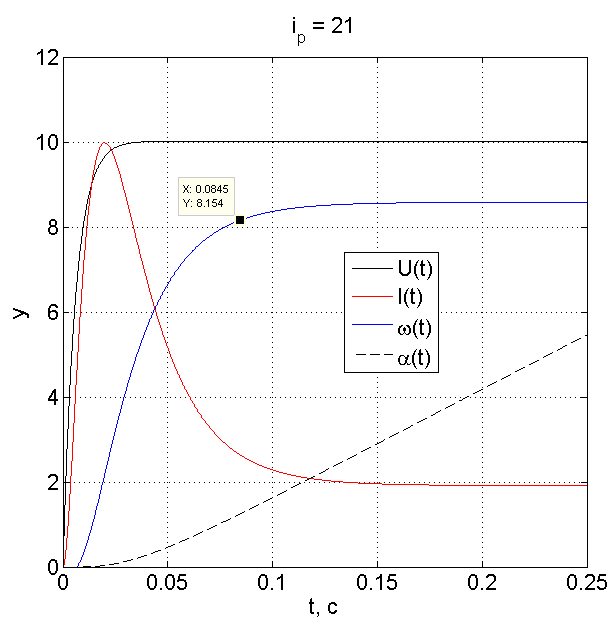
\includegraphics[width = \textwidth]{M44i21}
		\end{subfigure}
		\caption{Графики переходных процессов при ненулевом моменте сопротивления и при различных значениях передаточного момента редуктора}
		\label{M44ivar}
	\end{figure}

	На представленных результатах моделирования видно, что при наличии момента нагрузки и малом показателе передаточного момента редуктора система может не справиться с нагрузкой и никогда не прийти в устойчивое состояние. В нашем случае при значении $i_p = 3$ момента вращения двигателя не хватает, чтобы преодолеть момент сопротивления нагрузки. Так же можно наблюдать, что при увеличении $i_p$ не только уменьшаются значения времени переходного процесса и максимального тока, но и установившиеся значения угловой скорости и тока приближаются к значениям без нагрузки.
	\clearpage
	\section{Исследование влияния значений постоянных времени на вид переходных процессов}
	Для проведения данного исследования уменьшим заданные значения постоянных времени на порядок и получим
	\begin{align}
		T_\text{у} = 0,5 \text{мс} = 0,0005 c\\
		T_\text{я} = 0,6 \text{мс} = 0,0006 c
	\end{align}
	\begin{figure}[ht!]
		\centering
		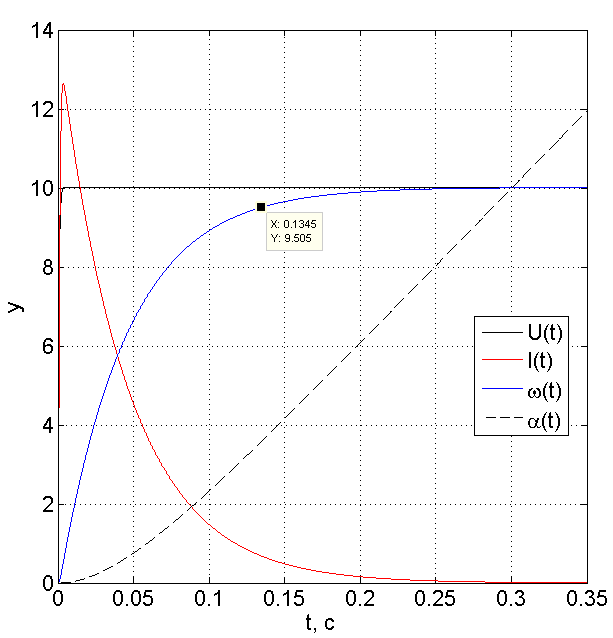
\includegraphics[width = 0.8\textwidth]{Tvar}
		\caption{График переходного процесса при уменьшенных значениях постоянных времени}
		\label{TVar}
	\end{figure}
	
	При уменьшении значений постоянных времени на порядок возросло максимальное значение тока. Время переходного процесса и установившиеся значения тока и скорости остались неизменны.
	\clearpage
	\section{Вывод математической модели Вход-Состояние-Выход для приближённой схемы моделирования электромеханического объекта}
	Для составления упрощённой модели ЭМО постоянные времени $T_\text{У}$ и $T_\text{Я}$ приравнивают к 0, так как их значение существенно меньше, чем значение механической постоянной времени $T_M$. Для получения упрощённой модели Вход-Состояние-Выход произведём соответствующие подстановки в уравнения для полной системы (\ref{ESETh}).
	\begin{align}
		&&\begin{cases}
			\dot{\omega} = -\displaystyle{\frac{K_MK_\text{Д}K_C}{J_\Sigma}}\omega + \frac{K_MK_\text{Д}K_C}{J_\Sigma}U - \frac{1}{J_\Sigma}M_C\\
			\dot{\alpha} = \omega
		\end{cases},
	\end{align}
	и на основании полученной системы построим модель:
	\begin{align}
		&&\begin{cases}
			\begin{bmatrix}
				\dot{\alpha}\\
				\dot{\omega}
			\end{bmatrix} =
			\begin{bmatrix}
				0 & 1\\
				0 & -\displaystyle{\frac{K_MK_\text{Д}K_C}{J_\Sigma}}
			\end{bmatrix}
			\begin{bmatrix}
				\alpha\\
				\omega
			\end{bmatrix} + 
			\begin{bmatrix}
				0 & 0\\
				\displaystyle{\frac{K_MK_\text{Д}K_E}{J_\Sigma}} & -\displaystyle{\frac{1}{J_\Sigma}}
			\end{bmatrix}
			\begin{bmatrix}
				U\\
				M_C
			\end{bmatrix}\\
			\alpha =
			\begin{bmatrix}
				1 & 0
			\end{bmatrix}
			\begin{bmatrix}
				\alpha\\
				\omega
			\end{bmatrix}
		\end{cases}.
	\end{align}
	
	Подставив значения, получим матрицы:
	\begin{align}
		&&A =
		\begin{bmatrix}
			0 & 1\\
			0 & -22,07
		\end{bmatrix}, B = 
		\begin{bmatrix}
			0 & 0\\
			22,07 & 78,99
		\end{bmatrix}
	\end{align}
	\clearpage	
	\section{Математическое моделирование приближённой модели электромеханического объекта}
	Составим упрощённую модель ЭМО на основе структурной схемы, представленной на рисунке \ref{simpScheme}.
	\begin{figure}[ht!]
		\centering
		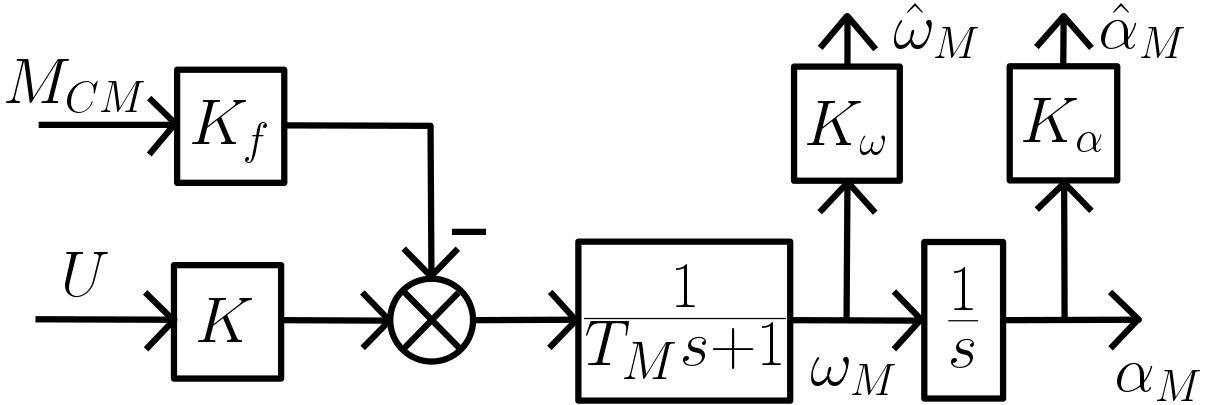
\includegraphics[width = 0.9\textwidth]{simpScheme}
		\caption{Структурная схема упрощённой модели ЭМО}
		\label{simpScheme}
	\end{figure}
	
	Рассчитаем параметры упрощённой ЭМО:
	\begin{align}
		K &= \frac{K_\text{у}}{K_E\cdot i_p} = \frac{4,8}{0,4583 \cdot 16} &= 0,6546\\
		K_f &= \frac{R}{K_M\cdot K_E\cdot i_p^2} = \frac{0,75}{0,4583\cdot0,4583\cdot16^2} &= 0,01395\\
		T_M &= \frac{R\cdot J_\Sigma}{K_M\cdot K_E} = \frac{0,75\cdot0,01266}{0,4583\cdot0,4583} &= 0,0452
	\end{align}
	
	На основе полученных параметров построим математическую модель упрощённой ЭМО. Схема модели приведена на рисунке \ref{simpModel}.
	\begin{figure}[ht!]
		\centering
		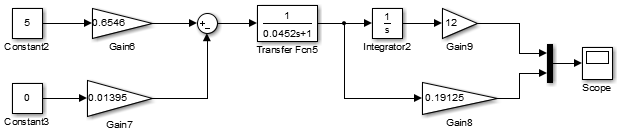
\includegraphics[width = \textwidth]{simpModel}
		\caption{Схема моделирования упрощённой ЭМО}
		\label{simpModel}
	\end{figure}
	\newpage
	Сравнение графиков переходных процессов по скорости полной и упрощённой моделей ЭМО приведёны на рисунке \ref{simpTP}.
	\begin{figure}[ht!]
		\centering
		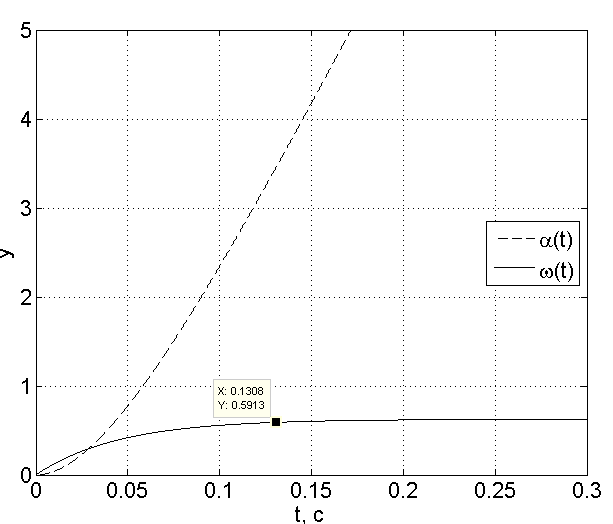
\includegraphics[width = 0.9\textwidth]{simpTP}
		\caption{График сравнения переходных процессов полной и упрощённой моделей ЭМО}
		\label{simpTP}
	\end{figure}
	
	Как можно заметить, время переходного процесса на обоих графиках совпадают, но есть различия в характере кривой.
	
	Так же проведём сравнение переходных процессов в полной и упрощённой моделях при меньших значениях постоянных времени $T_\text{У} = 6\cdot10^{-4}$ и $T_\text{Я} = 5\cdot10^{-4}$. Результаты сравнения приведены на рисунке.
	\begin{figure}[ht!]
		\centering
		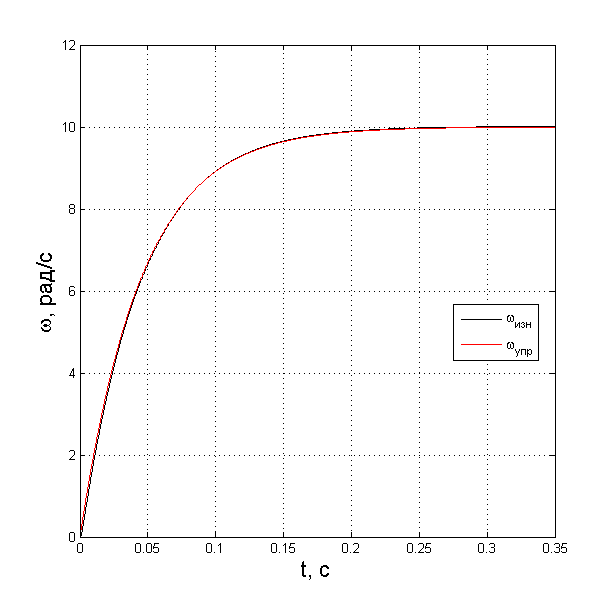
\includegraphics[width = 0.9\textwidth]{simpTvar}
		\caption{График сравнения переходных процессов полной и упрощённой моделей ЭМО при меньших значениях постоянных времени}
		\label{simpTvar}
	\end{figure}
	\newpage
	Как видно на рисунке \ref{simpTvar} различия между полной и упрощённой моделями становятся незначительными при уменьшении постоянных времени.
	\clearpage
	\section*{Вывод}
	В ходе работы было показано, как различные параметры, такие как момент сопротивления нагрузки, передаточный момент редуктора и постоянные времени влияют на показатели переходных процессов системы и её работоспособность в целом.
	
	Так же была исследована упрощённая модель электромеханического объекта и в ходе математического моделирования было показано, что её можно использовать при постоянных времени $T_\text{У}$ и $T_\text{Я}$ значительно меньших механической постоянной времени $T_M$.
\end{document}